% !TeX root = main.tex
%===================================== CHAP 2 =================================

\chapter{Background Theory}\label{chap:background-theory}

\section{The B-spline}
\label{sec:b-spline-theory}
This chapter will introduce B-splines, a type of spline function that is widely used in computer graphics, computer-aided design, and numerical optimization. B-splines are piecewise polynomial functions that are defined recursively in terms of a degree $p$ and a set of so-called knots. The chapter will cover the definition of B-splines, their properties, and common operations that can be performed on them. 

Important properties and operations on B-splines are presented, providing discussion and intuition around results and theorems without going into the full mathematical details. The goal is to provide the reader with the necessary background to understand the subsequent chapters in addition to being able to implement B-splines in a numerical optimization context from scratch.

\subsection{Definition and Properties}\label{sec:b-spline-definition}
The following definition is from \cite{Grimstad2016}:
A B-spline $f: \mathbb R \rightarrow \mathbb R$ is given by $n$ \emph{B-spline coefficients} $\mathbf c = [c_j]_{j=0}^{n-1}$ and $n+p+1$ non-decreasing knots $\mathbf t = [t_j]_{j=0}^{n+p}$ as follows:

\begin{equation}\label{eq:b-spline-def}
    f(x ; \mathbf{c}, p, \mathbf{t})=\sum_{j=0}^{n-1} c_j B_{j, p, \mathbf{t}}(x)=\mathbf{c}^{\top} \mathbf{B}_{\mathrm{p}, \mathrm{t}}(\mathrm{x})
\end{equation}

When the parameters $\mathbf{c}, p$, and $\mathbf{t}$ are given by the context, $f(x ; \mathbf{c}, p, \mathbf{t})$ is simply denoted $f(x)$. The sequence of coefficients $c_j$ control the shape of the B-spline, and the degree $p$ is a non-negative integer. The B-spline basis functions $B_{j, p, \mathbf{t}}(x)$ are defined recursively in terms of the degree $p$ and the knots $\mathbf t$ to form the column vector $\mathbf{B}_{p, \mathbf{t}}(x) = [B_{j, p, \mathbf{t}}(x)]_{j=0}^{n-1}$. 
in \cref{eq:b-spline-def}. These B-spline basis functions are defined as

\begin{subequations}\label{eq:b-spline-recurrence}
    \begin{align}
        B_{j, p, \mathbf{t}}(x) & =\frac{x-t_j}{t_{j+p}-t_j} B_{j, p-1, \mathrm{t}}(x)+\frac{t_{j+1+p}-x}{t_{j+1+p}-t_{j+1}} B_{j+1, p-1, \mathrm{t}}(x) \label{eq:b-spline-recurrence-p} \\
        B_{j, 0, \mathbf{t}}(x) & := 
        \mathbf 1_{[t_j, t_{j+1})} =
        \begin{cases}
            1, & t_j \leq x<t_{j+1} \\
            0, & \text { otherwise }
        \end{cases} \label{eq:b-spline-recurrence-0}
    \end{align}
\end{subequations}

From \cref{eq:b-spline-recurrence}, it is clear that the B-spline basis functions are all non-negative, as \cref{eq:b-spline-recurrence-0} gives $B_{j, 0, \mathbf{t}}(x) \geq 0 \quad\forall j, x$, and the coefficients $\frac{x-t_j}{t_{j+p}-t_j}$ and $\frac{t_{j+1+p}-x}{t_{j+1+p}-t_{j+1}}$
in \cref{eq:b-spline-recurrence-p} are also non-negative $\forall x, j\in[0,\dots,n-1], p, \mathbf t$ by the non-decreasing condition on the knots $\mathbf t$. 

\Cref{eq:b-spline-recurrence} also implies $B_{j, p, \mathbf{t}}(x)$ has local support on the interval $[t_j, t_{j+p+1})$. This can be seen by noting that the support of $B_{j, 0, \mathbf{t}}$, $\text{supp}(B_{j, 0, \mathbf{t}}) = [t_j, t_{j+1})$ and for each of the $p$ recurrence steps in \cref{eq:b-spline-recurrence-p}, the support is extended by one knot. 

It can also be shown that the B-spline basis functions are a partition of unity, i.e. $\sum_{j=0}^{n-1} B_{j, p, \mathbf{t}}(x) = 1 \quad\forall x \in [t_0, t_{n+p})$ \citep{deBoor1978practicalguide}.

These properties are well-documented in the literature and are summarized as follows:
\begin{property}[Nonnegativity]\label{b-prop:nonnegativity}
    $B_{j, p, \mathbf{t}}(x) \geq 0 \quad\forall j, p$, and $x$.
\end{property}

\begin{property}[Local support]\label{b-prop:localsupport}
    $B_{j, p, \mathbf{t}}(x)=0 \quad\forall x \notin [t_j, t_{j+p+1})$.
\end{property}

\begin{property}[Partition of unity]\label{b-prop:partitionofunity}
    $\sum_{j=i-p}^i B_{j, p, \mathbf{t}}(x)=1 \quad\forall x \in [t_i, t_{i+1})$.
\end{property}

So far, only B-splines with a one-dimensional co-domain have been considered. However, B-splines can be extended to curves in higher dimensions by simply allowing the coefficients $c_j$ to be vectors. In this case the B-spline is a vector-valued function $f: \mathbb R \rightarrow \mathbb R^m$. The \cref{b-prop:nonnegativity,b-prop:localsupport,b-prop:partitionofunity} still hold, as the basis functions themselves are still scalar-valued. 



\begin{figure}
    \centering
    \includesvg[width=0.8\textwidth]{fig/b-spline/knots + control points.svg}
    \caption{A 3rd degree B-spline (full) with 4 control points, knot vector \raggedright{$\mathbf t = [0, 0, 0, 0.5, 1, 1, 1]$} and corresponding control polygon (dashed).}
    \label{fig:b-spline-knots-control-points}
\end{figure}

Together, \cref{b-prop:nonnegativity,b-prop:partitionofunity} imply that the B-spline in \cref{eq:b-spline-def} is a convex combination of the coefficients $\mathbf c$. This means that the B-spline is always within the convex hull of the control points $\mathbf c$.

\begin{property}[Convex hull]\label{b-prop:convexhull}
    $f(x) \in \text{conv}(\mathbf{c})
    \quad\forall x$.
\end{property}

The convex hull $\text{conv}(\mathbf{c})$ of a set of points $\mathbf{c} = \{c_1, c_2, \ldots, c_n\}$ is defined as the set of all convex combinations of the points. Mathematically, it is given by:
\begin{equation}
    \text{conv}(\mathbf{c}) = \left\{ \sum_{i=1}^n \lambda_i c_i \mid \lambda_i \geq 0, \sum_{i=1}^n \lambda_i = 1 \right\}
\end{equation}

\begin{figure}
    \centering
    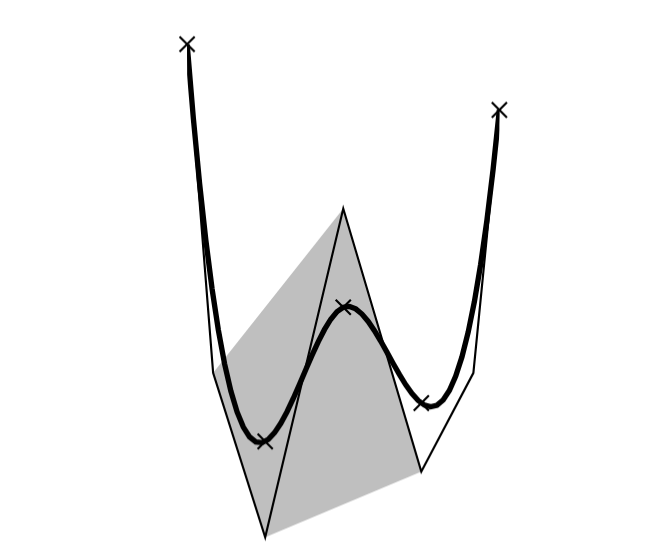
\includegraphics[width=0.8\textwidth]{fig/illustrations/convex-hull.png}
    \caption{A 3rd degree B-spline (full) with 4 control points (dots), control polygon (dashed) and convex hull (shaded area). The spline between the second and third control point (red) is always within the convex hull of the shaded area.}
    \label{fig:b-spline-convex-hull} 
\end{figure}
\todo{lag ny figur}
\todo{lag flere figurer}

In the context of optimization, this property is useful for formulating constraints, as a constraint on a B-spline function can be enforced by imposing them on the control points \citep{mercy2017spline}. 
\begin{equation}
    a \leq c_i \leq b \quad \forall i\in\{1,2,\ldots,n\} \implies a \leq f(x) \leq b \quad \forall x.
\end{equation}
Here $a$ and $b$ are constants of appropriate dimensions and the $\leq$ operator is applied element-wise.

The basis functions span a linear vector space (or spline space) denoted by $\mathcal{S}_{p, \mathbf{t}}$. This space contains all piecewise polynomials of degree $\le p$ on a given knot vector $\mathbf t$ \citep{Grimstad2016}. 

\subsection{Operations on B-splines}
From the recursive relation in \cref{eq:b-spline-recurrence} it follows that the B-spline basis functions are piecewise polynomial functions in $x$ of degree $p$. This property makes it clear that all polynomial operations on B-splines will result in a new B-spline.

In all following sections, it is assumed that for a given B-spline basis of degree $p$, the corresponding knot vector $\mathbf t$ is $p+1$ regular, i.e. all knots have multiplicity of most $p+1$ as well as the first and last knot having multiplicity $p+1$. The knot vector $\mathbf t$ can then be written with the notation 
\begin{equation}\label{eq:regular-knot-vector}
    \mathbf t = \{\underbrace{\eta_0, \dots, \eta_0}_{m_0}, \underbrace{\eta_1, \dots, \eta_1}_{m_1}, \dots, \underbrace{\eta_{r}, \dots, \eta_{r}}_{m_r}\} = \{\eta_0^{(m_0)}, \eta_1^{(m_1)}, \dots, \eta_r^{(m_r)}\}
\end{equation}
where $\{\eta_i\}$ is the set of unique knots in increasing order and $m_i$ denotes the multiplicity of the corresponding unique knot. For the knot vector to be regular, $m_0 = m_r = p+1$ and $m_i \leq p+1$ for $i \in \{1,2,\ldots,n-1\}$.

\subsection{Differentiation}\label{sec:derivative}
Given a B-spline $f(x) = \sum_{j=0}^{n-1} c_j B_{j, p, \mathbf{t}}(x)$,
the derivative of the B-spline can be computed by simply differencing its coefficients. 
\begin{equation}\label{eq:b-spline-derivative}
    \frac{d}{dx} f(x) = (p-1) \sum_{j=1}^{n-1} \frac{c_j-c_{j-1}}{t_{j+p-1}-t_j} B_{j, p-1, \boldsymbol{\tau}}(x)
\end{equation}
where $\boldsymbol{\tau} = [t_j]_{j=1}^{n+p-1}$ is the same knot vector as $\mathbf{t}$, but with the first and last knot removed in order to maintain \todo[inlinepar]{finn ord som passer}.

The new coefficients can be expressed using a transformation matrix $\mathbf T_D$ such that $\mathbf{c}_D = \mathbf T_D \mathbf{c}$, where $\mathbf{c}_D$ is the vector of coefficients of the derivative B-spline. The transformation matrix is then an $(n-1) \times n$ matrix with elements:

\begin{equation}
    \mathbf T_D = (p-1) \begin{bmatrix}
        -q_{1,p-1,\mathbf{t}}^{-1} & q_{1,p-1,\mathbf{t}}^{-1} & 0 & \cdots & 0 \\
        0 & -q_{2,p-1,\mathbf{t}}^{-1} & q_{2,p-1,\mathbf{t}}^{-1} & \cdots & 0 \\
        \vdots & \vdots & \vdots & \ddots & \vdots \\
        0 & \cdots & 0 & -q_{n-1,p-1,\mathbf{t}}^{-1} & q_{n-1,p-1,\mathbf{t}}^{-1} 
    \end{bmatrix},
\end{equation}
where $q_{j,p,\mathbf{t}} = (t_{j+p}-t_j)$.


The denominator $t_{j+p}-t_j$ in \cref{eq:b-spline-derivative} illustrates the continuity of the B-spline with respect to knot multiplicity. If a knot is repeated more than $p$ times, the denominator will be zero, and the derivative is not defined at that knot.

\subsection{Integration}
Given a degree $p$ and initial knot sequence $\mathbf t$, \cref{eq:b-spline-derivative}, gives
\begin{equation}\label{eq:b-spline-integral-pre}
    p \sum_{j=1}^{n-1} \gamma_j B_{j, p, \boldsymbol{t}}(x) 
    = \frac{d}{dx} \sum_{j=0}^{n-1} c_j B_{j, p+1, \boldsymbol{\tau}}(x),
\end{equation}
given that
\begin{equation}
    \gamma_j = \frac{c_j-c_{j-1}}{t_{j+p}-t_j},
\end{equation}
holds. Here, $\boldsymbol{\tau}$ is now the knot vector $\mathbf{t}$ with 1 additional knot at the beginning and end. Now
the new coefficients on the right hand side of \cref{eq:b-spline-integral-pre} can be expressed as 
\begin{equation}\label{eq:b-spline-integral-coefficients}
    c_j = c_{j-1} + \gamma_j \frac{t_{j+p}-t_j}{p}.
\end{equation}
This then gives the general anti-derivative of a B-spline as
\begin{equation}\label{eq:b-spline-integral}
    \int f(x) dx = \sum_{j=0}^{n-1} c_j B_{j, p+1, \boldsymbol{\tau}}(x)
\end{equation}
where $[c_j]_{j=1}^{n-1}$ are given by \cref{eq:b-spline-integral-coefficients}, $c_0$ is the constant of integration and $[\gamma_j]_1^{n-1}$ are the original coefficients of $f(x)$. In matrix form, the coefficients of the integral B-spline can be expressed as
\begin{equation}\label{eq:b-spline-integral-matrix}
    \mathbf{c}_I = \mathbf T_I \mathbf{c} + \mathbf{c}_0,
\end{equation}
where $\mathbf T_I$ is an $n \times (n-1)$ matrix with elements
\begin{equation}
    \mathbf T_I = \frac{1}{p}\begin{bmatrix}
        0 & 0 & \cdots & 0 \\
        q_{1,p,\mathbf{t}} & 0 & \cdots & 0 \\
        q_{1,p,\mathbf{t}} & q_{2,p,\mathbf{t}} & \cdots & 0 \\
        \vdots & \vdots & \ddots & \vdots \\
        q_{1,p,\mathbf{t}} & q_{2,p,\mathbf{t}} & \cdots & q_{n-1,p,\mathbf{t}}
    \end{bmatrix},\quad
    \mathbf{c}_0 = \begin{bmatrix}
        c_0 \\
        c_0 \\
        \vdots \\
        c_0
    \end{bmatrix}
\end{equation}

and $q_{j,p,\mathbf{t}} = (t_{j+p}-t_j)$ still.
As integration and differentiation are inverse operations, it should come as no surprise that the transformation matrices $\mathbf T_I$ and $\mathbf T_D$ are similirly related. This is explored further in \cref{app:homogeneous-integration-matrix}.


\subsection{Transforming Between Bases}\label{sec:basis-transformation}
In order to perform binary operations on spline functions such as multiplication and addition, it is necessary to be able to represent the same spline function in different bases. A powerful result from theory is that any spline function $\mathbf S$ expressed in a given basis $\mathbf B_{p,\mathbf t}$ can be represented in any other basis $\mathbf B_{q,\boldsymbol \tau}$ as long as $q \geq p$ and $\mathbf t \subseteq \boldsymbol \tau$\todo[inlinepar]{ikke helt sant} \citep{Grimstad2016}. Moreover, the coefficients in the new basis can be found by solving a linear system of equations. The following basis transformation method is employed in many algorithms in literature, and forms the foundation for the rest of the methods in this chapter, which is why a thorough explanation of this method is given attention here.

The goal is to find the transformation matrix $\mathbf T$ such that $\mathbf c_{q, \boldsymbol \tau} = \mathbf T \mathbf c_{p, \mathbf t}$, where $\mathbf c_{q, \boldsymbol \tau}$ and $\mathbf c_{p, \mathbf t}$ are the coefficients of the spline function $\mathbf S$ in the bases $\mathbf B_{q,\boldsymbol \tau}$ and $\mathbf B_{p,\mathbf t}$, respectively.

%The strategy to find $\mathbf T$ involves expressing the coefficients of the original basis $\mathbf c_{p, \mathbf t}$ as a linear combination of the refined basis $\mathbf c_{q,\boldsymbol \tau}$.
Noting that the two spline functions $\mathbf B_{q,\boldsymbol \tau}^\top \mathbf c_{q, \boldsymbol \tau}$, $\mathbf B_{p,\mathbf t}^\top \mathbf c_{p, \mathbf t}$ have to be equal,
the transformation matrix $\mathbf T$ can be found by sampling the B-spline basis functions at strategic points in the interval $[\tau_0, \tau_{n+q})$ to obtain a system of $m$ linear equations with $m$ unknowns.

The Greville abscissae $\boldsymbol \xi_{q,\boldsymbol \tau}=[\xi_{q,\boldsymbol \tau}]_{i=0}^{n-1}$ are a natural choice for the sampling points, as they represent the points at which the $i$-th basis function is most influential. 
They are given by the mean of the knots in each basis functions support $[\tau_i, \tau_{i+q+1})$ as
\begin{equation}\label{eq:greville-abscissae}
    \xi_{q,\boldsymbol \tau}(i) = \frac{1}{q+1} \sum_{j=i}^{i+q} \tau_j.
\end{equation}
The transformation matrix $\mathbf T$ can then be found by evaluating the B-spline basis functions at the Greville abscissae and solving the linear system of equations
\begin{equation}\label{eq:transformation-matrix-equation}
    \mathbf B_{q,\boldsymbol \tau}(\xi_{q,\boldsymbol \tau}(i))^\top \mathbf c_{q, \boldsymbol \tau} = \mathbf B_{p,\mathbf t}(\xi_{q,\boldsymbol \tau}(i))^\top \mathbf c_{p, \mathbf t} \quad \forall i\in\{0,1,\ldots,m-1\}
\end{equation}
for $\mathbf c_{q, \boldsymbol \tau}$. This can be written in matrix form as
\begin{equation}\label{eq:transformation-matrix}
    \underbrace{\begin{bmatrix}
        \mathbf B_{q,\boldsymbol \tau}(\xi_{q,\boldsymbol \tau}(0))^\top \\
        \mathbf B_{q,\boldsymbol \tau}(\xi_{q,\boldsymbol \tau}(1))^\top \\
        \vdots                                                             \\
        \mathbf B_{q,\boldsymbol \tau}(\xi_{q,\boldsymbol \tau}(m-1))^\top
    \end{bmatrix}}_{\mathbf A:\;m \times m}
    \underbrace{\begin{bmatrix}
        c_{q, \boldsymbol \tau, 0}   \\
        c_{q, \boldsymbol \tau, 1}   \\
        \vdots                       \\
        c_{q, \boldsymbol \tau, m-1} \\
    \end{bmatrix}}_{\mathbf c_{q,\boldsymbol\tau}:\;m \times 1}
    = 
    \underbrace{\begin{bmatrix}
        \mathbf B_{p,\mathbf t}(\xi_{q,\boldsymbol \tau}(0))^\top  \\
        \mathbf B_{p,\mathbf t}(\xi_{q,\boldsymbol \tau}(1))^\top  \\
        \vdots                                                       \\
        \mathbf B_{p,\mathbf t}(\xi_{q,\boldsymbol \tau}(m-1))^\top
    \end{bmatrix}}_{\mathbf D:\;m \times n}
    \underbrace{\begin{bmatrix}
        c_{p, \mathbf t, 0}   \\
        c_{p, \mathbf t, 1}   \\
        \vdots                \\
        c_{p, \mathbf t, n-1}
    \end{bmatrix}}_{\mathbf c_{p,\mathbf t}:\;n \times 1}
\end{equation}
or more compactly as
\begin{equation}
    [\mathbf B_{q,\boldsymbol \tau}(\boldsymbol \xi_{q,\boldsymbol \tau})^\top] \mathbf c_{q, \boldsymbol \tau} = [\mathbf B_{p,\mathbf t}(\boldsymbol \xi_{q,\boldsymbol \tau})^\top] \mathbf c_{p, \mathbf t}.
\end{equation}

The matrix $\mathbf T$ is then simply
\begin{equation}\label{eq:transformation-matrix-solution}
    \mathbf T = [\mathbf B_{q,\boldsymbol \tau}(\boldsymbol \xi_{q,\boldsymbol \tau})^\top]^{-1} [\mathbf B_{p,\mathbf t}(\boldsymbol \xi_{q,\boldsymbol \tau})^{\top}].
\end{equation}
As the B-spline basis functions are linearly independent, and the Greville abscissae are chosen such that each basis function is sampled at a point near the ``center'' of its support, the matrix $[\mathbf B_{q,\boldsymbol \tau}(\boldsymbol \xi_{q,\boldsymbol \tau})^\top]$ is always invertible. This method follows from the Schoenberg-Whitney Theorem \citep{schoenberg1988polya} for which a simple proof can be found in \cite{schoenberg2022proof}. The matrix $\mathbf A$ in \cref{eq:transformation-matrix} is known as a \emph{Collocation matrix} in the literature \todo[inlinepar]{Finn kilde} and can be used to interpolate an arbitrary function with a B-spline by replacing the right hand side of \cref{eq:transformation-matrix} with the function values sampled at the Greville abscissae.

\begin{algorithm}
    \caption{B-spline Basis Transformation}\label{alg:basis-transformation}
    \begin{algorithmic}[1]
        \State \textbf{Input:} B-spline basis $\mathbf{B}_{p,\mathbf{t}}$
        \State \textbf{Input:} Refined B-spline basis $\mathbf B_{q,\boldsymbol \tau}$
        \Ensure $q \geq p$
        \Ensure $\mathbf t \subseteq \boldsymbol \tau$
        \State $\boldsymbol \xi_{q, \boldsymbol \tau} \gets$ result from \cref{eq:greville-abscissae}
        \State $\mathbf A \gets [\mathbf B_{q,\boldsymbol \tau}(\boldsymbol \xi_{q,\boldsymbol \tau})^\top]$
        \State $\mathbf B \gets [\mathbf B_{p,\mathbf t}(\boldsymbol \xi_{q,\boldsymbol \tau})^\top]$
        \State $\mathbf T \gets \mathbf A^{-1} \mathbf B$
        \State \textbf{Output:} $\mathbf T$
    \end{algorithmic}
\end{algorithm}

\subsection{Knot Refinement and Degree Elevation}\label{sec:knot-refinement-degree-elevation}
The method in \cref{sec:basis-transformation} can be utilized for the two most commonly used techniques for manipulating B-splines: knot refinement and degree elevation. Knot refinement is simply the process of adding new knots to the knot vector, keeping the degree of the B-spline constant. 

Degree elevation, on the other hand, is the process of increasing the degree of the B-spline. There is a subtle caveat here, as the continuity of the B-spline at a knot is equal to the degree of the B-spline minus the multiplicity of the knot. This means that if a spline is to be represented in a higher degree basis, the knot multiplicity must be increased to maintain the same continuity at the knots. So, if a spline function in the basis $\mathbf B_{p,\mathbf t}$ is to be represented in the basis $\mathbf B_{p+1,\boldsymbol \tau}$, the knot vector $\boldsymbol \tau$ must contain the original knots $\mathbf t$ with multiplicity $p+1$.

In both knot refinement and degree elevation, the transformation matrix $\mathbf T$ from \cref{eq:transformation-matrix-solution} can be used to find the coefficients in the new basis. The following examples illustrate how to perform knot refinement and degree elevation on a B-spline.

$t = \{\underbrace{a, \dots, a}_{p+1}, \underbrace{\eta_1, \dots, \eta_1}_{m_1}, \dots, \underbrace{\eta_{n}, \dots, \eta_{n}}_{m_n}, \underbrace{b, \dots, b}_{p+1}\}$
$\mathbf u = \unique(x) = \{a, \eta_1, \dots, \eta_n, b\}$

\begin{algorithm}
    \caption{Degree Elevation}\label{alg:degree-elevation}
    \begin{algorithmic}[1]
        \State \textbf{Input:} Knot vector $\mathbf t = \{\eta_0^{(m_0)}, \eta_1^{(m_1)}, \dots, \eta_r^{(m_r)}\}$, degree $p$
        \State \textbf{Input:} Desired degree $q$
        \Ensure $q > p$
        \Ensure $m_0 = m_r = p+1$
        \Ensure $m_i \leq p+1$ for $i \in \{0,1,\ldots,r\}$
        \State $\boldsymbol\tau \gets \{\eta_0^{(m_0+p-q)}, \eta_1^{(m_1+p-q)}, \dots, \eta_r^{(m_r+p-q)}\}$
        \State $\mathbf T \gets $ result from \cref{alg:basis-transformation} with transformation from $\mathbf B_{p,\mathbf t}$ to $\mathbf B_{q,\boldsymbol \tau}$
        \State \textbf{Output:} $\mathbf B_{q, \boldsymbol \tau}, \mathbf T$
    \end{algorithmic}
\end{algorithm}

\begin{algorithm}
    \caption{Knot Refinement}\label{alg:knot-refinement}
    \begin{algorithmic}[1]
        \State \textbf{Input:} Knot vector $\mathbf t = \{\eta_0^{(m_0)}, \eta_1^{(m_1)}, \dots, \eta_r^{(m_r)}\}$, degree $p$
        \State \textbf{Input:} New knots to insert $\boldsymbol \xi = \{\xi_1, \xi_2, \dots, \xi_k\}$
        \Ensure $\xi_i \in (\eta_0, \eta_r)$
        \State $\boldsymbol \tau = \{\hat\eta_0^{(\hat m_0)}, \hat\eta_1^{(\hat m_1)}, \dots, \hat\eta_{\hat r}^{(\hat m_{\hat r})}\} \gets \mathbf t \cup_< \boldsymbol \xi$ \Comment{$\cup_<$ denotes the sorted union}
        \Ensure $\hat m_i \leq p+1$ for $i \in \{0,1,\ldots,\hat r\}$
        \State $\mathbf T \gets $ result from \cref{alg:basis-transformation} with transformation from $\mathbf B_{p,\mathbf t}$ to $\mathbf B_{p,\boldsymbol \tau}$
        \State \textbf{Output:} $\mathbf B_{p, \boldsymbol \tau}, \mathbf T$
    \end{algorithmic}
\end{algorithm}

\todo[inline]{legg til plot av konstant spline og lineær spline}
\begin{indentedexample}[Degree Elevation]
    We want to express the constant spline $f(x) =\mathbf B_{0, \mathbf t}^\top\mathbf c$ with knot vector $\mathbf t = \left[0, 1\right]$ as a linear spline $g(x) = \mathbf B_{1, \boldsymbol \tau}^\top \mathbf d$ with knot vector $\boldsymbol \tau = \left[0, 0, 1, 1\right]$. 

    The Greville abscissae for the linear spline are 
    \begin{equation*}
        \boldsymbol \xi_{1,\boldsymbol \tau} = 
        \begin{bmatrix}
            \frac{\tau_0 + \tau_1 + \tau_2}{3} &
            \frac{\tau_1 + \tau_2 + \tau_3}{3} 
        \end{bmatrix}
        =
        \begin{bmatrix}
            \frac{0 + 0 + 1}{3} & \frac{0 + 1 + 1}{3}
        \end{bmatrix} = \begin{bmatrix}
            \frac{1}{3} & \frac{2}{3}
        \end{bmatrix}.
    \end{equation*}
    Evaluating $\mathbf B_{0, \mathbf t}$ and $\mathbf B_{1, \boldsymbol \tau}$  at the Greville abscissae gives
    \begin{equation*}
        \begin{aligned}
            \mathbf B_{0, \mathbf t}\begin{pmatrix}\frac{1}{3}\end{pmatrix} &= \begin{bmatrix} 1 \end{bmatrix}, 
            &\mathbf B_{0, \mathbf t}\begin{pmatrix}\frac{2}{3}\end{pmatrix} &= \begin{bmatrix} 1 \end{bmatrix} 
            \\
            \mathbf B_{1, \boldsymbol \tau}\begin{pmatrix}\frac{1}{3}\end{pmatrix} &= \begin{bmatrix} \frac{2}{3} & \frac{1}{3} \end{bmatrix}^\top, 
            &\mathbf B_{1, \boldsymbol \tau}\begin{pmatrix}\frac{2}{3}\end{pmatrix} &= \begin{bmatrix} \frac{1}{3} & \frac{2}{3} \end{bmatrix}^\top
        \end{aligned}
    \end{equation*}
    Solving
    \begin{equation*}
        \begin{bmatrix}
            \frac{2}{3} & \frac{1}{3} \\
            \frac{1}{3} & \frac{2}{3}
        \end{bmatrix}
        \begin{bmatrix}
            d_0 \\
            d_1
        \end{bmatrix}
        =
        \begin{bmatrix}
            1 \\
            1
        \end{bmatrix}
        \begin{bmatrix}
            c_0
        \end{bmatrix}
    \end{equation*}
    gives the solution
    \begin{equation*}
        \begin{bmatrix}
            d_0 \\
            d_1
        \end{bmatrix}
        =
        \begin{bmatrix}
            2 & -1 \\
            -1 & 2
        \end{bmatrix}
        \begin{bmatrix}
            1 \\
            1
        \end{bmatrix}
        \begin{bmatrix}
            c_0
        \end{bmatrix}
        =
        \begin{bmatrix}
            1 \\
            1
        \end{bmatrix}
        \begin{bmatrix}
            c_0
        \end{bmatrix}
    \end{equation*}
\end{indentedexample}

\begin{indentedexample}[Knot Refinement]
    Given a linear spline function $f(x) = \mathbf B_{1, \mathbf t}^\top \mathbf c$ with knot vector $\mathbf t = \left\{ 0, 0, \frac{1}{2}, 1, 1\right\}$, the goal is to express it with in the basis $\mathbf B_{1, \boldsymbol \tau}$ with the refined knot vector $\boldsymbol \tau = \left\{ 0, 0, \frac{1}{4}, \frac{1}{2}, \frac{3}{4}, 1, 1\right\}$.

        The Greville abscissae for the refined basis are
        \begin{equation*}
            \boldsymbol \xi_{1,\boldsymbol \tau} = 
            \left\{
                \frac{1}{12}, \frac{3}{12}, \frac{6}{12}, \frac{9}{12}, \frac{11}{12}
            \right\}.
        \end{equation*}
        Using \cref{tab:linear-spline-evaluation} to evaluate $\mathbf B_{1,\boldsymbol\tau}(x)$ at the Greville abscissae gives
        \begin{equation*}
            \begin{aligned}
                \mathbf B_{1, \boldsymbol\tau}\begin{pmatrix}\frac{1}{12}\end{pmatrix} &= \begin{bmatrix} \frac{3}{4} & \frac{1}{4} & 0 & 0 & 0 \end{bmatrix}^\top,
                &\mathbf B_{1, \boldsymbol\tau}\begin{pmatrix}\frac{3}{12}\end{pmatrix} &= \begin{bmatrix} 0 & 1 & 0 & 0 & 0 \end{bmatrix}^\top, \\
                \mathbf B_{1, \boldsymbol\tau}\begin{pmatrix}\frac{6}{12}\end{pmatrix} &= \begin{bmatrix} 0 & 0 & 1 & 0 & 0 \end{bmatrix}^\top,
                &\mathbf B_{1, \boldsymbol\tau}\begin{pmatrix}\frac{9}{12}\end{pmatrix} &= \begin{bmatrix} 0 & 0 & 0 & 1 & 0 \end{bmatrix}^\top, \\
                \mathbf B_{1, \boldsymbol\tau}\begin{pmatrix}\frac{11}{12}\end{pmatrix} &= \begin{bmatrix} 0 & 0 & 0 & \frac{1}{4} & \frac{3}{4} \end{bmatrix}^\top,
            \end{aligned}
        \end{equation*}
        while evaluating $\mathbf B_{1,\mathbf t}(x)$ at the Greville abscissae gives
        \begin{equation*}
            \begin{aligned}
                \mathbf B_{1, \mathbf t}\begin{pmatrix}\frac{1}{12}\end{pmatrix} &= \begin{bmatrix} \frac{5}{6} & \frac{1}{6} & 0 \end{bmatrix}^\top,
                &\mathbf B_{1, \mathbf t}\begin{pmatrix}\frac{3}{12}\end{pmatrix} &= \begin{bmatrix} \frac{1}{2} & \frac{1}{2} & 0 \end{bmatrix}^\top, \\
                \mathbf B_{1, \mathbf t}\begin{pmatrix}\frac{6}{12}\end{pmatrix} &= \begin{bmatrix} 0 & 1 & 0 \end{bmatrix}^\top,
                &\mathbf B_{1, \mathbf t}\begin{pmatrix}\frac{9}{12}\end{pmatrix} &= \begin{bmatrix} 0 & \frac{1}{2} & \frac{1}{2} \end{bmatrix}^\top, \\
                \mathbf B_{1, \mathbf t}\begin{pmatrix}\frac{11}{12}\end{pmatrix} &= \begin{bmatrix} 0 & \frac{1}{6} & \frac{5}{6} \end{bmatrix}^\top.
            \end{aligned}
        \end{equation*}
        Inserting the calculated values into \cref{eq:transformation-matrix} gives
        \begin{equation*}
            \begin{bmatrix}
                \frac{3}{4} & \frac{1}{4} & 0 & 0 & 0 \\
                0 & 1 & 0 & 0 & 0 \\
                0 & 0 & 1 & 0 & 0 \\
                0 & 0 & 0 & 1 & 0 \\
                0 & 0 & 0 & \frac{1}{4} & \frac{3}{4}
            \end{bmatrix}
            \mathbf{d}
            =
            \begin{bmatrix}
                \frac{5}{6} & \frac{1}{6} & 0 \\
                \frac{1}{2} & \frac{1}{2} & 0 \\
                0 & 1 & 0 \\
                0 & \frac{1}{2} & \frac{1}{2} \\
                0 & \frac{1}{6} & \frac{5}{6}
            \end{bmatrix}
            \mathbf c,
        \end{equation*}
        which has the solution
        \begin{equation*}
            \mathbf d = \begin{bmatrix}
                \frac{8}{9} & \frac{1}{9} & 0 \\
                \frac{1}{2} & \frac{1}{2} & 0 \\
                0 & 1 & 0 \\
                0 & \frac{1}{2} & \frac{1}{2} \\
                0 & \frac{1}{9} & \frac{8}{9}
            \end{bmatrix}
            \mathbf c.
        \end{equation*}

            \centering
            \begin{tabular}{c|c|c|c|c|c}
                Knot Interval & $\mathbf B_{1, \boldsymbol\tau, 0}(x)$ & $\mathbf B_{1, \boldsymbol\tau, 1}(x)$ & $\mathbf B_{1, \boldsymbol\tau, 2}(x)$ & $\mathbf B_{1, \boldsymbol\tau, 3}(x)$ & $\mathbf B_{1, \boldsymbol\tau, 4}(x)$ \\[5pt]
                \hline
                \rule{0pt}{2.5ex} $\left[0,\frac{1}{4}\right]$ & $1-4x$ & $4x$ & 0 & 0 & 0 \\[5pt]
                \hline
                \rule{0pt}{2.5ex} $\left[\frac{1}{4},\frac{1}{2}\right]$ & 0 & $2-4x$ & $-1+4x$ & 0 & 0 \\[5pt]
                \hline
                \rule{0pt}{2.5ex} $\left[\frac{1}{2},\frac{3}{4}\right]$ & 0 & 0 & $3-4x$ & $-2+4x$ & 0 \\[5pt]
                \hline
                \rule{0pt}{2.5ex} $\left[\frac{3}{4},1\right]$ & 0 & 0 & 0 & $4-4x$ & $-3+4x$
            \end{tabular}
            \captionof{table}{The polynomials for each basis function in $\mathbf B_{1, \left[0, 0, \frac{1}{4}, \frac{1}{2}, \frac{3}{4}, 1, 1\right]}$ in their respecive knot intervals}
            \label{tab:linear-spline-evaluation}

\end{indentedexample}

\subsection{Addition and Subtraction}
Finding the sum of two B-splines that share the same basis is a simple task as their coefficients can just be added together:
\begin{equation}
    f(x) + g(x) =  \mathbf{B}_{p, \mathbf{t}}^{\top}(x) \mathbf{c}_1 + \mathbf{B}_{p, \mathbf{t}}^{\top}(x) \mathbf{c}_2
    = \mathbf{B}_{p, \mathbf{t}}^{\top}(x)(\mathbf{c}_1 + \mathbf{c}_2)
\end{equation}
If the spline functions are in different bases, however, they must be transformed to a common basis before the addition can be performed. So, for spline functions $f(x) = \mathbf{B}_{p_1, \mathbf{t}_1}^{\top}(x) \mathbf{c}_1$ and $g(x) = \mathbf{B}_{p_2, \mathbf{t}_2}^{\top}(x) \mathbf{c}_2$, with degrees $p_1$ and $p_2$ and knot vectors $\mathbf{t}_1$ and $\mathbf{t}_2$, the goal is to find a common basis $\mathbf{B}_{q, \boldsymbol{\tau}}^{\top}(x)$ with degree $q$ and knot vector $\boldsymbol{\tau}$ such that $h(x) = \mathbf{B}_{q, \boldsymbol{\tau}}^{\top}(x) \mathbf{d} = f(x) + g(x)$.

To do this, the basis of the lowest degree is first elevated to the highest degree, before the knot vectors are refined to a common knot vector. The transformation matrices $\mathbf T_1$ and $\mathbf T_2$ from the original bases to the common basis are then found using \cref{eq:transformation-matrix-solution}. The new coefficients $\mathbf d$ are then given by
\begin{equation}
    \mathbf d = \mathbf T_1 \mathbf c_1 + \mathbf T_2 \mathbf c_2.
\end{equation}

\begin{algorithm}
    \caption{Common Basis}\label{alg:common-basis}
    \begin{algorithmic}[1]
        \State \textbf{Input:} B-Spline basis functions $\mathbf{B}_{p_1, \mathbf{t}_1}^{\top}(x)$ and $\mathbf{B}_{p_2, \mathbf{t}_2}^{\top}(x)$
        \State \textbf{Input:} Desired degree $q$
        \Ensure $q \geq \max(p_1, p_2)$
        \State $\mathbf B_{q, \boldsymbol{\tau_1}} \gets$ result from \cref{alg:degree-elevation} with basis $\mathbf{B}_{p_1, \mathbf{t}_1}$ and degree $q$
        \State $\mathbf B_{q, \boldsymbol{\tau_2}} \gets$ result from \cref{alg:degree-elevation} with basis $\mathbf{B}_{p_2, \mathbf{t}_2}$ and degree $q$
        \State $\boldsymbol{\tau} \gets$ union of $\boldsymbol{\tau_1}$ and $\boldsymbol{\tau_2}$ with multiplicity for each knot set to the maximum of the two knot vectors
        \State \textbf{Output:} $\mathbf B_{q, \boldsymbol{\tau}}^{\top}(x)$
    \end{algorithmic}
\end{algorithm}


\begin{algorithm}
    \caption{Addition}\label{alg:addition}
    \begin{algorithmic}[1]
        \State \textbf{Input:} Spline functions $f(x) = \mathbf{B}_{p_1, \mathbf{t}_1}^{\top}(x) \mathbf{c}_1$ and $g(x) = \mathbf{B}_{p_2, \mathbf{t}_2}^{\top}(x) \mathbf{c}_2$
        \State $q \gets \max(p_1, p_2)$
        \State $\mathbf B_{q, \boldsymbol{\tau}} \gets $ result from \cref{alg:common-basis} with bases $\mathbf{B}_{p_1, \mathbf{t}_1}^{\top}(x)$ and $\mathbf{B}_{p_2, \mathbf{t}_2}^{\top}(x)$ and desired degree $q$
        \State $\mathbf T_1 \gets $ result from \cref{alg:basis-transformation} with transformation from $\mathbf B_{p_1, \mathbf{t}_1}$ to $\mathbf B_{q, \boldsymbol{\tau}}$
        \State $\mathbf T_2 \gets $ result from \cref{alg:basis-transformation} with transformation from $\mathbf B_{p_2, \mathbf{t}_2}$ to $\mathbf B_{q, \boldsymbol{\tau}}$
        \State \textbf{Output:} $\mathbf B_{q, \boldsymbol{\tau}}(x), \quad\mathbf T_1 \mathbf c_1 + \mathbf T_2 \mathbf c_2$
    \end{algorithmic}
\end{algorithm}

Scalar addition in the form of $f(x) + a$ can be performed by simply adding the scalar to all the coefficients of the B-spline. This is clear from the fact thats a scalar can be represented as a B-spline with degree $0$ (constant spline), and then performing the addition as described above. 

\subsection{Multiplication and Inner Product}\label{sec:multiplication}

For addition, the common basis had to have degree $q \geq \max(p_1, p_2)$, but for multiplication, the degree of the common basis must be $q = p_1 + p_2$\todo[inlinepar]{forklar hvorfor}. Intuitively, this is because the product of two polynomials of degree $p_1$ and $p_2$ will have degree of at most $p_1 + p_2$ while the sum of two polynomials of degree $p_1$ and $p_2$ will have degree of at most $\max(p_1, p_2)$.

In order to find the product of two B-splines, an approach similar to \cref{sec:basis-transformation} can be used. Given two spline functions $f(x) = \mathbf{B}_{p_1, \mathbf{t}_1}^{\top}(x) \mathbf{c}_1$ and $g(x) = \mathbf{B}_{p_2, \mathbf{t}_2}^{\top}(x) \mathbf{c}_2$, the goal is to find a common basis $\mathbf{B}_{q, \boldsymbol{\tau}}^{\top}(x)$ with degree $q$ and knot vector $\boldsymbol{\tau}$ such that $h(x) = \mathbf{B}_{q, \boldsymbol{\tau}}^{\top}(x) \mathbf{d} = f(x)  g(x)$.

Writing the equation for the product of the two B-splines gives
\begin{subequations}\label{eq:b-spline-product}
    \begin{align}
        h(x) &= f(x) g(x) \label{eq:b-spline-product-1} \\
        &= \left(\mathbf{B}_{p_1, \mathbf{t}_1}^{\top}(x) \mathbf{c}_1\right) 
        \left(\mathbf{B}_{p_2, \mathbf{t}_2}^{\top}(x) \mathbf{c}_2\right) \label{eq:b-spline-product-2} \\
        &= \left(\mathbf{B}_{p_1, \mathbf{t}_1}^{\top}(x) \otimes \mathbf{B}_{p_2, \mathbf{t}_2}^{\top}(x)\right) 
        \left(\mathbf{c}_1 \otimes \mathbf{c}_2\right) \label{eq:b-spline-product-3} \\
        \mathbf{B}_{q, \boldsymbol{\tau}}^{\top}(x) \mathbf{d} 
        &= \left(\mathbf{B}_{p_1, \mathbf{t}_1}(x) \otimes \mathbf{B}_{p_2, \mathbf{t}_2}(x)\right)^{\top} \left(\mathbf{c}_1 \otimes \mathbf{c}_2\right), \label{eq:b-spline-product-4}
    \end{align}
\end{subequations}

where $\otimes$ denotes the Kronecker product. In \cref{eq:b-spline-product-3}, the mixed product property of the Kronecker product has been used, while \cref{eq:b-spline-product-4} is obtained using the fact that the transpose is distributive over the Kronecker product \citep{LOAN200085}. \Cref{eq:b-spline-product-4} resembles the structure in \cref{eq:transformation-matrix-equation}, and the transformation matrix $\mathbf T$ from $\mathbf c_1 \otimes \mathbf c_2$ to $\mathbf d$ can similarily be found by sampling \cref{eq:b-spline-product-4} at the Greville abscissae of $\mathbf B_{q, \boldsymbol{\tau}}^{\top}(x)$. This is summarized in \cref{alg:multiplication}.

This algorithm can be made more efficient by exploiting the local support property of B-splines. The product of two B-splines is zero outside the union of the supports of the two B-splines, and the transformation matrix $\mathbf T$ will have many zero entries. So, instead of computing the Kronecker products $\mathbf B_{p_1, \mathbf{t}_1}(x) \otimes \mathbf B_{p_2, \mathbf{t}_2}(x)$ and $\mathbf c_1 \otimes \mathbf c_2$, which are column vectors of $p_1\cdot p_2$ entries, one can instead create vectors where only the non-zero entries of $\mathbf B_{p_1, \mathbf{t}_1}(x) \otimes \mathbf B_{p_2, \mathbf{t}_2}(x)$ and corresponding entries of $\mathbf c_1 \otimes \mathbf c_2$ are stored. 

\begin{algorithm}
    \caption{Product}\label{alg:multiplication}
    \begin{algorithmic}[1]
        \State \textbf{Input:} Spline functions $f(x) = \mathbf{B}_{p_1, \mathbf{t}_1}^{\top}(x) \mathbf{c}_1$ and $g(x) = \mathbf{B}_{p_2, \mathbf{t}_2}^{\top}(x) \mathbf{c}_2$
        \State $q \gets p_1 + p_2$
        \State $\mathbf B_{q, \boldsymbol{\tau}} \gets $ result from \cref{alg:common-basis} with bases $\mathbf{B}_{p_1, \mathbf{t}_1}^{\top}(x)$ and $\mathbf{B}_{p_2, \mathbf{t}_2}^{\top}(x)$ and desired degree $q$
        \State $\mathbf T \gets $ result from \cref{alg:basis-transformation} with transformation from $\mathbf B_{p_1, \mathbf{t}_1}^{\top}(x) \otimes \mathbf B_{p_2, \mathbf{t}_2}^{\top}(x)$ to $\mathbf B_{q, \boldsymbol{\tau}}^{\top}(x)$
        \State \textbf{Output:} $\mathbf B_{q, \boldsymbol{\tau}}(x), \quad\mathbf T (\mathbf c_1 \otimes \mathbf c_2)$
    \end{algorithmic}
\end{algorithm}


\begin{indentedexample}[B-Spline Product]
    \label{ex:linear-spline-multiplication}
    Consider the two B-splines
    \begin{equation*}
        f(x) = \mathbf{B}_{p_1, \mathbf t_1}^\top(x) \mathbf{c}_1
        \quad g(x) = \mathbf{B}_{p_2, \mathbf t_2}^\top(x) \mathbf{c}_2
    \end{equation*}
    with knot vectors $\mathbf t_1 = \left\{0, 0, \frac{1}{3}, \frac{2}{3}, 1, 1\right\}$,  $\mathbf t_2 = \left\{0, 0, 0, \frac{1}{4}, \frac{1}{2}, \frac{3}{4}, 1, 1, 1\right\}$ and degrees  $p_1 = 1$, $p_2 = 2$. 
    The common basis $\mathbf{B}_{q,\boldsymbol{\tau}}$ is then found using \cref{alg:common-basis}, to get:
    \begin{equation*}
        q = p_1 + p_2 = 3,
        \quad
        \boldsymbol{\tau} = \left\{0, 0, 0, 0, \frac{1}{4}, \frac{1}{4}, \frac{1}{3}, \frac{1}{3}, \frac{1}{3}, \frac{1}{2}, \frac{1}{2}, \frac{2}{3}, \frac{2}{3}, \frac{2}{3}, \frac{3}{4}, \frac{3}{4}, 1, 1, 1, 1\right\},
    \end{equation*}
    where the internal knots of $\mathbf t_1$ and $\mathbf t_2$ have been duplicated twice and once respectively to account for the degree elevation. 
    The left hand side of \cref{eq:b-spline-product-4} is found as in \cref{eq:transformation-matrix}, sampling $\mathbf B_{q, \boldsymbol{\tau}}(x)$ at the Greville abscissae $\boldsymbol{\zeta_\tau}$.
    For the right hand side, we can write out the product of the B-splines in matrix form using the Kronecker product:
    \begin{equation*}
        \begin{aligned}
            (\mathbf B_{p_1, \mathbf{t}_1}(\boldsymbol{\zeta_\tau}) \otimes \mathbf B_{p_2, \mathbf{t}_2}(\boldsymbol{\zeta_\tau}))^\top \mathbf{c}_1 \otimes \mathbf{c}_2 = \begin{bmatrix}
                B_{0, p_1, \mathbf{t}_1}(\boldsymbol{\zeta_\tau}) B_{0, p_2, \mathbf{t}_2}(\boldsymbol{\zeta_\tau}) \\
                B_{0, p_1, \mathbf{t}_1}(\boldsymbol{\zeta_\tau}) B_{1, p_2, \mathbf{t}_2}(\boldsymbol{\zeta_\tau}) \\
                B_{0, p_1, \mathbf{t}_1}(\boldsymbol{\zeta_\tau}) B_{2, p_2, \mathbf{t}_2}(\boldsymbol{\zeta_\tau}) \\
                \vdots \\
                B_{0, p_1, \mathbf{t}_1}(\boldsymbol{\zeta_\tau}) B_{m, p_2, \mathbf{t}_2}(\boldsymbol{\zeta_\tau}) \\
                B_{1, p_1, \mathbf{t}_1}(\boldsymbol{\zeta_\tau}) B_{0, p_2, \mathbf{t}_2}(\boldsymbol{\zeta_\tau}) \\
                \vdots \\
                B_{n, p_1, \mathbf{t}_1}(\boldsymbol{\zeta_\tau}) B_{m, p_2, \mathbf{t}_2}(\boldsymbol{\zeta_\tau}) \\
            \end{bmatrix}^\top 
            \begin{bmatrix}
                c_{0, 1} c_{0, 2} \\
                c_{0, 1} c_{1, 2} \\
                c_{0, 1} c_{2, 2} \\
                \vdots \\
                c_{0, 1} c_{m, 2} \\
                c_{1, 1} c_{0, 2} \\
                \vdots \\
                c_{n, 1} c_{m, 2}
            \end{bmatrix}                
        \end{aligned}
    \end{equation*}
    This is a matrix with $p_1 \cdot p_2$ rows and column number equal to the number of Greville abscissae in $\boldsymbol{\tau}$, which depend on the degrees of $\mathbf B_{p_1, \mathbf{t}_1}$ and $\mathbf B_{p_2, \mathbf{t}_2}$ and how many knots they share.
    In order to save computational resources, the products with non-overlapping supports should be ignored. In this example the supports of the two B-splines are given in \cref{tab:ex-spline-supports}. Here we only get 6 zero-entries, but as the knot vectors get denser, this number will increase.


    \centering
    \small
    \begin{tabular}{c|c||c|c|c|c|c|c}
        \textbf{Basis} &  & $B_{0, p_2, \mathbf{t}_2}$ & $B_{1, p_2, \mathbf{t}_2}$ & $B_{2, p_2, \mathbf{t}_2}$ & $B_{3, p_2, \mathbf{t}_2}$ & $B_{4, p_2, \mathbf{t}_2}$ & $B_{5, p_2, \mathbf{t}_2}$ \\[5pt]
        \hline
        \rule{0pt}{2.5ex} & \textbf{Support} & $\left[0, \frac{1}{4}\right]$ & $\left[0, \frac{1}{2}\right]$ & $\left[0, \frac{3}{4}\right]$ & $\left[\frac{1}{4}, \frac{3}{4}\right]$ & $\left[\frac{1}{2}, 1\right]$ & $\left[\frac{3}{4}, 1\right]$ \\[5pt]
        \hline\hline
        \rule{0pt}{2.5ex}$B_{0, p_1, \mathbf{t}_1}$ & $\left[0, \frac{1}{3}\right]$ & 
        1 & 1 & 1 & 1 & 0 & 0 \\[5pt]\hline\rule{0pt}{2.5ex}
        $B_{0, p_1, \mathbf{t}_1}$ & $\left[0, \frac{2}{3}\right]$ &
        1 & 1 & 1 & 1 & 1 & 0 \\[5pt]\hline\rule{0pt}{2.5ex}
        $B_{2, p_1, \mathbf{t}_1}$ & $\left[\frac{1}{3}, 1\right]$ &
        0 & 1 & 1 & 1 & 1 & 1 \\[5pt]\hline\rule{0pt}{2.5ex}
        $B_{2, p_1, \mathbf{t}_1}$ & $\left[\frac{2}{3}, 1\right]$ & 
        0 & 0 & 1 & 1 & 1 & 1 \\[5pt]
    \end{tabular}
    \captionof{table}{Overlapping supports of $B_{p_1, \mathbf{t}_1}$ and $B_{p_2, \mathbf{t}_2}$ in \cref{ex:linear-spline-multiplication}.}
    \label{tab:ex-spline-supports}

\end{indentedexample}

The inner product of two (vector-valued) functions is a scalar that measures the similarity between the functions. combines the components of the two vector-valued functions. This operation is useful in applications such as calculating projections, or defining cost functions in optimization problems. The $\mathcal L_2$ inner product (henceforth referred to as the inner product)for vector-valued functions is defined as:
\begin{equation}
    \label{eq:dot-product}
    \langle\mathbf f(x), \mathbf g(x)\rangle = \int_{-\infty}^\infty\sum_{i=1}^m f_i(x) g_i(x)
\end{equation}
where $\mathbf f, \mathbf g: \mathbb{R} \to \mathbb{R}^m$, $\mathbf f(x) = [f_1(x), \ldots, f_m(x)]^\top$ and $\mathbf g(x) = [g_1(x), \ldots, g_m(x)]^\top$ are vector-valued functions with $m$ components. The expression inside the integral also carries useful information, and one may refer to it as the pointwise (PW) inner product which is defined as
\begin{equation}
    \label{eq:dot-product-pointwise}
    \mathbf f(x) \cdot \mathbf g(x) = \sum_{i=1}^m f_i(x) g_i(x).
\end{equation}

When $\mathbf f$ and $\mathbf g$ are spline functions, the PW inner product can be expressed in terms of their B-spline representations as
\begin{equation}
    \label{eq:dot-product-spline}
    \begin{aligned}
        \langle\mathbf f(x), \mathbf g(x)\rangle &= \langle\mathbf B_{p_1, \mathbf t_1}^\top(x) \mathbf c_1, \mathbf B_{p_2, \mathbf t_2}^\top(x) \mathbf c_2\rangle \\
        &= \sum_{i=1}^m \left(\mathbf B_{p_1, \mathbf t_1}^\top(x) \mathbf c_{1,i}\right) \left(\mathbf B_{p_2, \mathbf t_2}^\top(x) \mathbf c_{2,i}\right) \\
        &= \sum_{i=1}^m \left(\mathbf B_{p_1, \mathbf t_1}^\top(x) \otimes \mathbf B_{p_2, \mathbf t_2}^\top(x)\right) \left(\mathbf c_{1,i} \otimes \mathbf c_{2,i}\right) \\
        &= \left(\mathbf B_{p_1, \mathbf t_1}(x) \otimes \mathbf B_{p_2, \mathbf t_2}(x)\right)^{\top} \sum_{i=1}^m \mathbf c_{1,i} \otimes \mathbf c_{2,i},
    \end{aligned}
\end{equation}
where $\mathbf c_{1,i}$ and $\mathbf c_{2,i}$ are the coefficients of the $i$-th component of $\mathbf f$ and $\mathbf g$, respectively. Notice that the expression $\left(\mathbf B_{p_1, \mathbf t_1}(x) \otimes \mathbf B_{p_2, \mathbf t_2}(x)\right)^{\top}$ is found in both \cref{eq:b-spline-product-4} and \cref{eq:dot-product-spline}. This means that the transformation matrix $\mathbf T$ for the inner product can be computed in the same way as for the multiplication, using \cref{alg:multiplication}.
This is due to the fact that per \cref{eq:transformation-matrix-solution}, the transformation matrix $\mathbf T$ is independent of the coefficients $\mathbf c_{1}$ and $\mathbf c_{2}$.

So, to find the PW inner product $h(x) = \mathbf f(x) \cdot \mathbf g(x)$, \cref{alg:multiplication} is used on the bases of $\mathbf f$ and $\mathbf g$, and the coefficients $\mathbf d$ of $h(x) = \mathbf B_{q, \boldsymbol{\tau}}^\top(x) \mathbf d$ are given by
\begin{equation}
    \mathbf d = \mathbf T \sum_{i=1}^m (\mathbf c_{1,i} \otimes \mathbf c_{2,i}).
\end{equation}

As for the regular product, the PW inner product can be made more efficient by not computing the terms in the Kronecker product that correspond to non-overlapping supports of the basis functions. The most common case for applying the PW inner product is between two vector-valued B-splines of the same basis, in which case the number of non-zero entires is $n(p+1)$, where $n$ is the number of basis functions and $p$ is the degree of the B-spline. This is linear in the number of basis functions, instead of quadratic as for when this optimization is not used. See explanation in \cref{fig:overlapping-bases}. Finding a general formula arbitrary bases is not as easily acheivable, as the number of non-zero entries depends on the placement of the knots in the knot vectors.

\begin{figure}
    \centering
    \includesvg[width=\textwidth,pretex=\footnotesize]{fig/b-spline/overlapping-bases.svg}
    \caption{The overlapping supports of the B-splines. Each rectangle represents the support of a basis function, so counting the number of basis functions withing each knot interval gives the number of multiplications for that interval. The total number of multiplications then the area of all the rectangles, which is $n(p+1)$, where $n$ is the number of basis functions and $p$ is the degree of the B-spline.}
    \label{fig:overlapping-bases}
\end{figure}


\subsection{Pythogerean-Hodograph B-splines (PH B-Splines)}\label{sec:pythogerean-hodograph}
The Pythogerean-Hodograph (PH) B-spline is utilized to leverage exact geometric quantities in CAD/CAM. Pythagorean‐Hodograph (PH) B‐splines \cite{Albrecht2016}, a natural extension of PH Bézier curves \cite{Farouki1990}, are employed. In this framework, the hodograph (derivative) 
\begin{equation*}
    \mathbf r'(x) = [a'(x), b'(x)]
\end{equation*}
of a planar B‐spline
\begin{equation*}
    \mathbf r(x) = [a(x), b(x)],
\end{equation*}
satisfies the Pythagorean condition
\begin{equation}\label{eq:pythagorean-condition}
a'(x)^2 + b'(x)^2 = \sigma(x)^2,
\end{equation}
where $\sigma(x)$ is itself a B‐spline function. Enforcing \cref{eq:pythagorean-condition} guarantees that magnitude, curvature, turn‐rate, and arc‐length admit closed‐form rational expressions without numerical approximation. The following derivation is based on \cite{Albrecht2016}.

Introducing the complex pre‐image
\begin{equation*}
    z(x) = u(x) + i\,v(x),
\end{equation*}
the hodograph is defined via the square relation
\begin{equation}\label{eq:hodograph-square}
    \mathbf r'(x) = z(x)^2.
\end{equation}
Expanding the complex square yields
\begin{equation*}
    (u + i v)^2 = u^2 + 2iuv - v^2 = (u^2 - v^2) + i(2uv),
\end{equation*}
and equating real and imaginary parts gives
\begin{subequations}\label{eq:hodograph-derivatives}
    \begin{align}
        a'(x) &= \Re\bigl(z(x)^2\bigr) = u(x)^2 - v(x)^2, \label{eq:hodograph-derivatives-a}\\
        b'(x) &= \Im\bigl(z(x)^2\bigr) = 2\,u(x)\,v(x), \label{eq:hodograph-derivatives-b}
    \end{align}
\end{subequations}
while the magnitude of the hodograph follows as
\begin{equation*}
    \sigma(x) = \|\mathbf r'(x)\| = |z(x)|^2 = u(x)^2 + v(x)^2.
\end{equation*}
Finally, integrating recovers the curve coordinates:
\begin{equation*}
    \begin{aligned}
        a(x) &= a_0 + \int_{x_0}^{x}\bigl(u(\tau)^2 - v(\tau)^2\bigr)\,d\tau,\\
        b(x) &= b_0 + \int_{x_0}^{x}2\,u(\tau)\,v(\tau)\,d\tau,
    \end{aligned}
\end{equation*}

where $(a_0,b_0)=\mathbf r(x_0)$.

The curvature $\kappa(x)$ of the curve $\mathbf r(x)$ is defined as
\begin{equation*}
    \kappa(x) = \frac{a'(x)b''(x) - b'(x)a''(x)}{\|\mathbf r'(x)\|^3},
\end{equation*}
where $a'(x)$ and $b'(x)$ are the first derivatives of the curve, and $a''(x)$ and $b''(x)$ are the second derivatives. Using \cref{eq:hodograph-derivatives} gives
which in terms of $u(x)$ and $v(x)$ simplifies to
\begin{equation}\label{eq:curvature}
    \kappa(x) = \frac{2(uv'-vu')}{(u^2+v^2)^2}.
\end{equation}
The turn-rate $\dot\theta(x)$ is then
\begin{equation}\label{eq:turn-rate}
    \dot\theta(x) = \kappa(x) \sigma(x) = \frac{2(uv'-vu')}{u^2+v^2},
\end{equation}
while the arc-length $s(x)$ is given by
\begin{equation*}
    s(x) = \int_{x_0}^{x}\sigma(\tau)\,d\tau.
\end{equation*}


\subsection{Non-Uniform Rational B-splines (NURBS)}
In the previous section, rational functions of B-splines were mentioned in the context of Pythagorean-Hodograph curves. \Cref{eq:curvature,eq:turn-rate} are examples of such rational functions. This section formalizes the concept of Non-uniform rational B-splines (NURBS), for which a good reference is \cite{Piegl1997}. 

NURBS are defined by the rational basis functions
\begin{equation}\label{eq:nurbs-basis}
R_{i,p,\mathbf t, \mathbf w}(x)  = \frac{w_i,B_{i,p,\mathbf t}(x)}{\sum_{j=0}^{n-1}w_j,B_{j,p,\mathbf t}(x)},
\end{equation}
for which a NURBS curve is given by
\begin{equation}\label{eq:nurbs-curve}
\mathbf r(x; \mathbf c, p, \mathbf t, \mathbf w)  = \sum_{i=0}^{n-1}R_{i,p,\mathbf t, \mathbf w}(x)\,c_i
= \mathbf R_{p,\mathbf t, \mathbf w}(x)^\top \mathbf c.
\end{equation}

NURBS inherit the local support and non-negativity properties from B-splines. When all weights $w_i$ are equal, the NURBS reduces exactly to a B-spline curve. The partition of unity property is also preserved as long as all the weights are non-negative. \citep{Piegl1997}

A principal advantage of NURBS is their ability to represent conic sections — such as circles, ellipses, and parabolas exactly using quadratic or cubic segments \citep{Piegl1997}. For example, a circle can be constructed by appropriate choice of four rational quadratic segments, each representing a quarter arc \citep{DenbighStarkeyNURBS}. Many CAD systems likewise rely on NURBS for the exactness of the conic-surface representation as well as the ability to create flexible free-form shapes \citep{Farin1991,PieglTillerSIGGRAPH,cottrell2009isogeometric}.

In \cref{sec:b-spline-definition} it is mentioned that a B-spline function $f(x; p, \mathbf t)$ is part of the linear vector space $\mathbb S_{p, \mathbf t}$.
, a NURBS function $f(x; p, \mathbf t, \mathbf w)$ is part of the rational spline space $\mathbb B_{p, \mathbf t, \mathbf w}$. This space contains all piecewise rational polynomials on the knot vector $\mathbf t$ with degree $p$ and weights $\mathbf w$. 

To convert a general rational B-spline
$$
    f(x) = \frac{N(x)}{D(x)},
$$
where $N(x)=\mathbf B_{p_N,\mathbf t_N}^\top\mathbf n$ and $D(x)=\mathbf B_{p_D,\mathbf t_D}^\top\mathbf d$ are each in separate B-spline bases, into the standard NURBS form, one applies degree elevation and knot insertion \citep{Piegl1997} to obtain a common basis ${B_{q,i}(x)}$:
\begin{enumerate}
    \item Elevate both $N$ and $D$ to degree $q\ge\max{p_N,p_D}$ using \cref{alg:degree-elevation}.
    \item Refine knot vectors so that both share the same sequence using \cref{alg:knot-refinement}.
\end{enumerate}
This yields
$$
    \widetilde N(x) = \sum_{i=0}^M \tilde n_i\,N_{q,i}(x),\quad \widetilde D(x) = \sum_{i=0}^M \tilde d_i\,N_{q,i}(x),
$$
from which the NURBS weights and control values follow:
$$
    w_i = \tilde d_i, \quad
    c_i = \frac{\tilde n_i}{\tilde d_i}.
$$
The resulting representation,
$$
    f(x) = \frac{\sum_i w_i\,c_i\,N_{q,i}(x)}{\sum_i w_i\,N_{q,i}(x)},
$$
is a degree-$q$ NURBS with weights $w_i$, knot vector $\boldsymbol{\tau}$ and control points $c_i$. This is summarized in \cref{alg:nurbs-conversion}.

\begin{algorithm}
    \caption{Convert rational B-spline to NURBS}\label{alg:nurbs-conversion}
    \begin{algorithmic}[1]
        \State \textbf{Input:} B-splines $N(x)$ and $D(x)$ with correspondingknot vectors $\mathbf t_N$ and $\mathbf t_D$, and degrees $p_N$ and $p_D$
        \State $q \gets \max(p_N, p_D)$
        \State $\mathbf B_{q,\boldsymbol{\tau}}(x) \gets $ result from \cref{alg:common-basis} with bases $\mathbf B_{p_N,\mathbf t_N}(x)$ and $\mathbf B_{p_D,\mathbf t_D}(x)$ and desired degree $q$
        \State $\mathbf T_N \gets $ result from \cref{alg:basis-transformation} with transformation from $\mathbf B_{p_N,\mathbf t_N}(x)$ to $\mathbf B_{q,\boldsymbol{\tau}}(x)$
        \State $\mathbf T_D \gets $ result from \cref{alg:basis-transformation} with transformation from $\mathbf B_{p_D,\mathbf t_D}(x)$ to $\mathbf B_{q,\boldsymbol{\tau}}(x)$
        \State $\mathbf{\tilde n} \gets \mathbf T_N \mathbf n$
        \State $\mathbf{\tilde d} \gets \mathbf T_D \mathbf d$
        \State $\mathbf w \gets \mathbf{\tilde d}$
        \State $\mathbf c \gets \mathbf{\tilde n} \oslash \mathbf{\tilde d}$ \Comment{element-wise division}
        \State \textbf{Output:} Degree $q$ NURBS curve $\displaystyle r(x) = \frac{N(x)}{D(x)}$ with weights $w_i$, knot vector $\boldsymbol{\tau}$ and control points $c_i$
    \end{algorithmic}
\end{algorithm}


\subsection{Summary}

This chapter has introduced the concept of B-splines, their properties, and how they can be used to represent curves and surfaces. B-splines are piecewise polynomial functions defined over a knot vector, and they have several important properties, including local support, non-negativity, and the ability to represent complex shapes. The chapter also discussed the operations of addition, multiplication, and inner product for B-splines, as well as their generalization to Non-Uniform Rational B-splines (NURBS).

Table of operations for B-splines is given in \cref{tab:operations}. A summary of operations on \acrshort{NURBS} can be found in \cite{piegl1997symbolic}.


\renewcommand{\arraystretch}{1.2}
\begin{table}
    \centering
    \small
    \begin{tabular}{|l|l|l|l|c|}
    \hline
    \textbf{Operation} 
      & \textbf{Expression} 
        & \textbf{Space} 
          & \textbf{Coefficients} 
            & \textbf{Reference} \\
    \hline
    \hline
    Evaluation   
      & $\mathbf f(x)$ 
        & $\mathbb S^n_{p}\to\mathbb{R}^n$ 
          & Linear 
            & \cref{eq:b-spline-recurrence} \\
    \hline
    Derivative   
      & $\mathbf f'$  
        & $\mathbb S^n_{p}\to\mathbb S^n_{p-1}$ 
          & Linear 
            & \cref{eq:b-spline-derivative} \\
    \hline
    Integral     
      & \rule{0pt}{4ex}$\displaystyle\int \mathbf f(x)\,dx$ 
        & $\mathbb S^n_{p}\to\mathbb S^n_{p+1}$ 
          & Linear 
            & \cref{eq:b-spline-integral} \\[1.5ex]
    \hline
    Degree elevation  
      & $\mathbf f$  
        & $\mathbb S^n_{p}\to\mathbb S^n_{p+1}$ 
          & Linear 
            & \Cref{alg:degree-elevation} \\      
    \hline
    Knot insertion    
      & $\mathbf f$  
        & $\mathbb S^n_{p}\to\mathbb S^n_{p}$ 
          & Linear 
            & \Cref{alg:knot-refinement} \\
    \hline
    \hline
    Vector Addition  
      & $\mathbf a + \mathbf f$  
        & $\mathbb R^n \times\mathbb S^n_{p}\to\mathbb S^n_{p}$ 
          & Linear 
            & \Cref{alg:addition} \\
    \hline
    Scalar multiplication  
      & $a\,\mathbf f$  
        & $\mathbb R\times\mathbb S^n_{p}\to\mathbb S^n_{p}$ 
          & Linear 
            & $-$ \\
    \hline
    Addition     
      & $\mathbf f +\mathbf g$  
        & $\mathbb S^n_{p_1}\times\mathbb S^n_{p_2}\to\mathbb S^n_{\max(p_1,p_2)}$ 
          & Linear 
            & \Cref{alg:addition} \\[.5ex]
    \hline
    Multiplication   
      & $\mathbf f\,g$  
        & $\mathbb S^n_{p_1}\times\mathbb S_{p_2}\to\mathbb S^n_{p_1+p_2}$ 
          & Bilinear 
            & \Cref{alg:multiplication} \\
    \hline
    PW inner product  
      & $\mathbf f \cdot \mathbf g$  
        & $\mathbb S^n_{p_1}\times\mathbb S^n_{p_2}\to\mathbb S_{p_1+p_2}$
          & Bilinear 
            & \cref{eq:dot-product-pointwise} \\
    \hline
    Inner product    
      & $\langle \mathbf f, \mathbf g \rangle$  
        & $\mathbb S^n_{p_1}\times\mathbb S^n_{p_2}\to\mathbb R$ 
          & Bilinear 
            & \cref{eq:dot-product} \\
    \hline
    Division  
      & \rule{0pt}{4ex}$\displaystyle\frac{\mathbf f}{g}$  
        & $\mathbb S^n_{p_1}\times\mathbb S_{p_2}\to\mathbb B^n_{\max(p_1,p_2)}$
          & Rational 
            & \Cref{alg:nurbs-conversion} \\[1.5ex]
    \hline
    \end{tabular}
    \caption{Summary of B-spline operations and their properties. The symbols $f$ and $g$ denote B-spline functions, while $a$ denotes a scalar. Their corresponding bold-faced symbols denote vector-valued functions and vectors in $\mathbf R^n$ space respectively. The ``Coefficients'' column indicates the transformation type of the operation on the coefficients. The ``Space'' column indicates the space of the resulting B-spline. The knot vectors for these spaces are ommited for brevity and can be found in the references in the ``Algorithms'' column.}
    \label{tab:operations}
\end{table}
\renewcommand{\arraystretch}{1}
    